%!Mode:: "TeX:UTF-8"
%!TEX encoding = UTF-8 Unicode
%language = en
%arara: xelatex
\documentclass{ctexart}
\newcommand{\Kappa}{\mathrm{K}}
\newcommand{\argmin}{\mathrm{argmin}}
\newif\ifpreface
%\prefacetrue
\input{../../../global/all}
\begin{document}
\large
\setlength{\baselineskip}{1.2em}
\ifpreface
\input{../../../global/preface}
\newgeometry{left=2cm,right=2cm,top=2cm,bottom=2cm}
\else
\newgeometry{left=2cm,right=2cm,top=2cm,bottom=2cm}
\maketitle
\fi
%from_here_to_type

\begin{problem}\label{pro:1}
  \(H_{n + 1,n} \) is the Hessenberg matrix of Arnoldi process, which is executed for \(A \) and \(b \) at step \(n \).
  If \(h_{N + 1,N} =0\), then
  \begin{enumerate}
    \item \(\Kappa_N(A,b) \) is \(A- \) invariant subspace.
    \item \(\Kappa_n(A,b)=\Kappa_{n + 1}(A,b), n \geq N \).
    \item \(\sigma(H_N) \subset \sigma(A) \), where \(\sigma(M) \) is the eigenvalue set of matrix \(M \).
    \item If \(A \) is nonsigular, the solution of the equation \(Ax=b \) lies in \(\Kappa_N(A,b) \).
  \end{enumerate}
\end{problem}
\begin{solution}
  Assume \(Q_n =(q_1,\cdots,q_n)\) at step \(n \) in Arnoldi process.
  \begin{enumerate}
    \item Since \(K_{N + 1}(A,b)=span\{b,\cdots,A^Nb\}=span\{b,AK_N(A,b)\} \), we only need to prove \(AK_N(A,b) \subset K_N(A,b) \).
      Since \(AQ_n=Q_{n + 1} H_{n + 1,n} \) exists for all step \(n \) and \(H_{N + 1,N}=0 \), we can get \(AQ_N=Q_N H_{N} + h_{N + 1,N}q_{N + 1} e_N^T \), where \(e_N \)
      is unit vector with only one none zero element at position \(N \). Thus,
      \begin{equation}\label{equ:*}
        AQ_N=Q_N H_N .
      \end{equation}
      Besides, \(\{q_1,\cdots,q_N\} \) is the base of space \(K_N(A,q) \), so \(span\{Aq_1,\cdots,A_{N}\} = A K_N(A,b) =span(Q_N H_N)\subset K_N(A,q) \).
    \item First, we can prove \(K_{n}(A,b) \subset K_{N}(A,b), n \geq N \). We will use MI to prove. \(n=N \), this property holds, obviously.
      Assume \(K_t(A,b) \subset K_N (A,b) \) for some \(t \geq N \), then \(K_{t + 1}(A,b)=span\{b,AK_t(A,b)\} \).
      Besides, \(K_N(A,b) \) is \(A \)- invariant subspace, then \(A K_t(A,b) \subset A K_N(A,b) \subset K_N(A,b) \).
      Thus, \(K_{t + 1}(A,b) \subset K_N(A,b) \).

      Since \(K_n(A,b) =span\{b,\cdots,A^{n-1}b\} \supset span\{b,\cdots,A^{N-1}b\}=K_N(A,b) \), we can get \(K_n(A,b)=K_N(A,b) ,\forall n \geq N\).
    \item Assume \(\lambda \) is the eigenvalue of \(H_N \) with eigenvector \(u \), then \(H_N u=\lambda u \).
      By \eqref{equ:*}, \(AQ_N u=Q_N H_N u= \lambda  Q_N u \), therefore, \(\lambda \) is an eigenvalue of \(A \) with eigenvector \(Q_N u \).
    \item We only need to prove \(\res{A}{K_N(A,b)}: K_N(A,b) \to K_N(A,b)\) is bijective. Since \(K_N(A,b) \) is \(A \)-invariant, we can get \(\res{A}{K_N(A,b)} \) well-defined.
      \(\forall y \in K_N(A,b), Ay =0 \), then \(y=0 \) due to the reversibility of A.
      Thus, \(Ker(\res{A}{K_N(A,b)})=0 \), then \(\res{A}{K_N(A,b)}\) is injective.
      Since \(\{q_1,\cdots,q_N\} \) are base of \(K_N(A,b) \), we can get \(\sum_{i=1}^{N}c_iq_i=0 \iff c_i=0, 1 \leq i \leq N \). Then \(\sum_{i=1}^{N}d_i Aq_i=A(\sum_{i=1}^{N}d_i q_i)=0 \iff \sum_{i=1}^{N} d_i q_i =0 \iff d_i=0, 1 \leq i \leq N \).
      Then, \(\{Aq_1,\cdots,Aq_N\} \) are base of \(K_N(A,b) \).
      We can get that \(\forall y \in K_N(A,b) \), \(y=\sum_{i=1}^{N} a_i Aq_i=A \sum_{i=1}^{N}a_iq_i=Ax \), where \(x= \sum_{i=1}^{N}a_iq_i \). So \(\res{A}{K_N(A,b)} \) is surjective.
      Just let \(y=b \), the equation has solution in \(K_N(A,b) \).
  \end{enumerate}
\end{solution}
\begin{problem}\label{pro:2}
  Let \(A \in \mathbb{C}^{m \times m}\), \(b \in \mathbb{C}^m\), and \(p \in \mathcal{P}_n\).
  Suppose that we want to compute \(p(A)b\). A natural place to start is with Horner’s rule, which can be written as
  \begin{equation}\label{equ:2}
    p(z) = c_0 + z\bigl(c_1 + z(c_2 + \cdots + z(c_{n-1} + z c_n)\cdots)\bigr).
  \end{equation}

  \begin{enumerate}[label=(\alph*)]
    \item Write a \texttt{for} loop based on \eqref{equ:2} (on paper, not on a computer) that computes \(p(A)\) and then applies the result to \(b\). Determine the number of flops required by this algorithm, to leading order.

    \item Write another \texttt{for} loop for computing \(p(A)b\), a far better one, in which \(b\) is introduced into the process at the beginning. Again determine the number of flops required to leading order.

    \item In introductory numerical analysis texts, Horner’s rule is recommended for evaluation of polynomials because it is faster than the obvious method of computing powers \(z^k\), multiplying by coefficients \(c_k\), and adding. Show that for computing \(p(A)\) or \(p(A)b\), by contrast, Horner’s rule is not significantly faster than the obvious method.
  \end{enumerate}
\end{problem}
% \begin{solution}
%   \begin{enumerate}
%     \item First version are as befow:
%       \begin{algorithm}
%         \caption{Horner method for $p(A)b$}
%         \begin{algorithmic}
%           \State $P \gets c_n I_m$
%           \For{$k = n-1, n-2, \dots, 0$}
%           \State $P \gets A P + c_k I_m$
%           \EndFor
%           \State \(y \leftarrow Pb  \)
%           \State \Return $y$
%         \end{algorithmic}
%       \end{algorithm}
%       At each iteration, we compute \(P \leftarrow AP + c_k I_m \), which has \(((m+(m - 1))\times m)\times m + m = 2m\)
%       flops, so we have \((2m^3 -m^2 +m)\times n \) flops, which has \(O(2m^3n) \) leading order.
%   \end{enumerate}
%%TODU:
\begin{solution}
  \begin{enumerate}[label=(\alph*)]
    \item A straightforward implementation of Horner's rule for first computing
      \(p(A)\) and then applying it to \(b\) is:

      \begin{algorithm}
        \caption{Horner method for computing \(p(A)\) and then \(p(A)b\)}
        \begin{algorithmic}
          \State \(P \gets c_n I_m\)
          \For{\(k = n-1, n-2, \dots, 0\)}
          \State \(P \gets AP + c_k I_m\)
          \EndFor
          \State \(y \gets Pb\)
          \State \Return \(y\)
        \end{algorithmic}
      \end{algorithm}

      At each step of the loop, the dominant operation is the matrix--matrix
      product \(AP\), which costs \(2m^3 + O(m^2)\) flops. The addition
      \(c_k I_m\) changes only the diagonal entries, so it costs only \(m\) flops.
      Thus each iteration costs
      \[
        2m^3 + O(m^2)
      \]
      flops, and over \(n\) iterations the total cost is
      \[
        2nm^3 + O(nm^2).
      \]
      Finally, multiplying \(P\) by \(b\) costs \(2m^2 + O(m)\) flops. Therefore
      the total number of flops is
      \[
        2nm^3 + O(nm^2),
      \]
      so to leading order the algorithm requires
      \[
        \boxed{2nm^3 \text{ flops}.}
      \]

    \item A much better algorithm is to introduce \(b\) at the beginning and
      evaluate \(p(A)b\) directly:

      \begin{algorithm}
        \caption{Horner method for directly computing \(p(A)b\)}
        \begin{algorithmic}
          \State \(y \gets c_n b\)
          \For{\(k = n-1, n-2, \dots, 0\)}
          \State \(y \gets Ay + c_k b\)
          \EndFor
          \State \Return \(y\)
        \end{algorithmic}
      \end{algorithm}

      Now the dominant operation in each iteration is the matrix--vector product
      \(Ay\), which costs \(2m^2 + O(m)\) flops. The vector update \(y + c_k b\)
      costs only \(O(m)\) flops. Hence each iteration costs
      \[
        2m^2 + O(m)
      \]
      flops, and after \(n\) iterations the total is
      \[
        2nm^2 + O(nm).
      \]
      Thus, to leading order, this algorithm requires
      \[
        \boxed{2nm^2 \text{ flops}.}
      \]

      This is far better than part (a), since it reduces the cost from order
      \(m^3\) per step to order \(m^2\) per step.

    \item The ``obvious'' method for computing \(p(A)\) is to form the powers
      \(A^k\), multiply each by \(c_k\), and add:
      \[
        p(A) = c_0 I + c_1 A + c_2 A^2 + \cdots + c_n A^n.
      \]
      This requires computing the powers \(A^2, A^3, \dots, A^n\), which involves
      \(n-1\) matrix--matrix multiplications. Since each such multiplication costs
      \(2m^3 + O(m^2)\) flops, the total cost is again
      \[
        2nm^3 + O(nm^2),
      \]
      i.e.,
      \[
        \boxed{O(nm^3)}
      \]
      to leading order. Therefore Horner's rule is not significantly faster than
      the obvious method for computing \(p(A)\): both have the same leading-order
      cost.

      Likewise, the obvious method for computing \(p(A)b\) is to form the vectors
      \[
        b,\ Ab,\ A^2b,\ \dots,\ A^n b
      \]
      recursively, and then combine them:
      \[
        p(A)b = c_0 b + c_1 Ab + c_2 A^2b + \cdots + c_n A^n b.
      \]
      Computing \(A^k b\) successively requires \(n\) matrix--vector products, each
      costing \(2m^2 + O(m)\) flops, so the total cost is
      \[
        2nm^2 + O(nm),
      \]
      i.e.,
      \[
        \boxed{O(nm^2)}
      \]
      to leading order. This is the same leading-order cost as the Horner method
      in part (b).

      Hence, unlike the scalar case, Horner's rule is not significantly faster than
      the obvious method when computing \(p(A)\) or \(p(A)b\). The reason is that
      in the matrix setting the dominant cost comes from matrix--matrix or
      matrix--vector multiplications, and both approaches require essentially the
      same number of such expensive operations.
  \end{enumerate}
\end{solution}

\begin{problem}\label{pro:3}
  \(H \in \mathbb{C}^{m xm}  \) is a Hessenberg matrix, \(f \) is a polynomial with degree \(n<m \), \(H_n \in \mathbb{C}^{n x n}\) is the first matrix block of \(H \).
  Then \(f(H) \) and \(f(H_n) \) has same \(n \) entries in the first column.
\end{problem}
\begin{solution}
  Since \(A=QHQ^*\), we have
  \[
    p_n(A)b = Qp_n(H)Q^*b.
  \]
  Because \(q_1=b/\norm{b}\), it follows that
  \[
    Q^*b=\norm{b}e_1.
  \]
  Hence
  \[
    Q_n^*p_n(A)b
    = \norm{b}\,Q_n^*Q\,p_n(H)e_1
    = \norm{b}\,[I_n\ 0]\,p_n(H)e_1.
  \]
  Therefore \(Q_n^*p_n(A)b=0\) if and only if the first \(n\) entries of the first column of \(p_n(H)\) are zero.

  Now write
  \[
    p_n(z)=\sum_{k=0}^n a_k z^k.
  \]
  Since \(H\) is upper Hessenberg, for each \(k\le n\), the first \(n\) entries of \(H^k e_1\) depend only on the leading principal block \(H_n\), and equal \(H_n^k e_1\). Therefore
  \[
    [I_n\ 0]\,p_n(H)e_1
    =
    \sum_{k=0}^n a_k [I_n\ 0]\,H^k e_1
    =
    \sum_{k=0}^n a_k H_n^k e_1
    =
    p_n(H_n)e_1.
  \]
  Thus the first \(n\) entries of the first column of \(p_n(H)\) are exactly the first \(n\) entries of the first column of \(p_n(H_n)\).
\end{solution}
\begin{problem}\label{pro:4}
  Assume \(H_n \) at step \(n \) in Arnoldi process, the Ritz values of \(H_n \) are eigenvalues of \(H_n \).
  \begin{enumerate}
    \item If \(A \) is changed to \(A + \sigma I \),\(\sigma \in \mathbb{C} \),\(b \) is unchanged, then the Ritz values \(\{\theta_j\} \) are changed to \(\{\theta_j + \sigma\} \).
    \item If \(A \) is changed to \(\sigma A \),\(\sigma \in \mathbb{C}\setminus\{0\} \),\(b \) is unchanged, then the Ritz values \(\{\theta_j\} \) are changed to \(\{\sigma \theta_j\} \).
    \item \(U^* U =I \), if \(A \) is changed to \(U A U^*\),\(b \) is changed to \(Ub \), then the Ritz values \(\{\theta_j\} \) don't change.
  \end{enumerate}
\end{problem}
\begin{solution}
  \begin{enumerate}
    \item Since \((A + \sigma I)^k =\sum_{t=0}^{k} a_t A^t \subset K_n(A,b), 1 \leq k \leq n\), we can get that \(K_n(A + \sigma I,b)=span\{b,(A + \sigma I)b,\cdots,(A + \sigma I)^{n-1} b\}\subset span\{b,Ab,\cdots,A^{n -1} b\}=K_n(A,b) \).
      Besides, \((A + \sigma I - \sigma I)=A \), then \(K_n((A + \sigma I)-\sigma I, b) \subset K_n(A + \sigma I, b) \) holds for the same reason.
      Thus, \(K_n(A + \sigma I,b)=K_n(A,b) \). Assume \( Q_n, H_n\) be the responding matrix in Arnoldi process executed by \(A  \) and \(b \) at step \(n \).
      So \(Q_n \) is the orthonormal basis of \(K_n(A + \sigma I,b) \).
      Then \( AQ_n=Q_{n + 1} H_{n + 1}=Q_n H_n + h_{n + 1,n} q_{n + 1} e_n^T\), then \(Q_n^* A Q_n =Q_n^* Q_n H_n +  h_{n + 1,n}Q_n^*q_{n + 1} e_n^T=H_n\). Then \(\tilde{H_n}=Q_n^*(A + \sigma I)Q_n=Q_n^*AQ_n + \sigma I=H_n + \sigma I \), where
      \(\tilde{H_n} \) is the representation matrix of \(K_n(A + \sigma I,b) \) in base \(Q_n \).

      Assume \(f \) be the characteristic polynomial of \(H_n \), \(\tilde{f} \) be the characteristic polynoimal of \(\tilde{H_n} \).
      So \(f(\lambda)= |H_n-\lambda I|= |\tilde{H_n} -\sigma I -\lambda I|=\tilde{f}(\lambda + \sigma) \). Thus, \(\theta \) be the Ritz of \(H_n \),
      then \(f(\theta )=0=\tilde{f}(\theta + \sigma) \).
      Then \(\theta + \sigma \) is the Ritz of \(\tilde{H_n} \).
    \item Since \((\sigma A)^k =\sigma^k A^k \in K_n(A,b), 1 \leq k \leq n \), we can get that \(K_n(\sigma A,b)=span\{b,\sigma A b,\cdots,(\sigma A)^{n-1}b\} \subset K_n(A,b)\) .
      Besides, \(\sigma^{-1}(\sigma A) =A \), then \(K_n(\sigma^{-1}(\sigma A),b) \subset K_n(\sigma A,b) \) holds for the same reason.
      Thus, \(K_n(\sigma A,b)=K_n(A,b) \). In the same reason as above, we can get \(\tilde{H_n}=Q_n^*(\sigma A)Q_n=\sigma H_n \), where \(\tilde{H_n} \)
      is the representation matrix of \(K_n(\sigma A,b) \) in orthonormal basis \(Q_n \).

      Assume \(f \) be the characteristic polynomial of \(H_n \), \(\tilde{f} \) be the characteristic polynoial of \(\tilde{H_n} \).
      So \(f(\lambda)=|H_n -\lambda I|=|(\sigma)^{-1} (\tilde{H_n} -\sigma \lambda I)|=\sigma^{-n}|\tilde{H_n} -\sigma \lambda I|=\sigma^{-n}  \tilde{f}(\sigma \lambda)\).
      Thus, \(\theta \) be the Ritz of \(H_n \), then \(f(\theta)=0=\sigma^{-n}\tilde{f}(\sigma \theta)\). Then \(\tilde{\sigma \theta}=0 \).
      Then \(\sigma \theta \) is the Ritz of \(\tilde{H_n} \).
    \item Since \((UAU^*)^k(Ub)=UA^kU^*Ub=UA^kb \), then \( K_n(UAU^*,Ub)=UK_n(A,b)\). Besides, \(U \) is reversible, so \(U Q_n \) is orthonormal matrix.
      Thus, \(UQ_n \) is the orthonormal basis of \(K_n(UAU^*,Ub) \). Then \(\tilde{H_n}=(UQ_n)^*(UAU^*)(UQ_n)=Q_n^*AQ_n =H_n \).
      Then, Ritz values don't change.
  \end{enumerate}
\end{solution}

\begin{problem}\label{pro:5}
  \(P_n:=\{1+\sum_{i=1}^{n} c_i z^i:c_i \in \mathbb{C}, 1 \leq i \leq n\} \), \(q=\argmin_{p \in P_n} \norm{p(A)b} \), \(r= q(A)b \).
  \begin{enumerate}
    \item If \(A  \) changed to \(\sigma A \),\(\sigma \in \mathbb{C} \setminus\{0\} \),\(b \) is changed to \(\sigma b \), then \(r \) is changed to \(r \).
    \item \(U^* U =I \), if \(A \) is changed to \(U A U^*\),\(b \) is changed to \(Ub \), then \(r \) changed to \(Ur \).
  \end{enumerate}
\end{problem}
\begin{solution}
  \begin{enumerate}
    \item Assume \(Q_n:=\{\sigma p(\sigma z): p \in P_n\} \), \(f: P_n \to Q_n, p(z) \mapsto \sigma p(\sigma z)\). We prove that \(f \) is bijective.
      Obviously, \(f \) is well-defined and surjective. Only need to prove \(f \) is injective.
      If \(\sigma p(\sigma z) =\sigma q(\sigma z) \), then \(p(\sigma z)=q(\sigma z) \). Thus, \(p(z)=q(z) \), which means \(f \) is injective.
      Since \(q =\argmin_{p \in P_n} \norm{p(A)b}\) and \(q(A)b= \sigma^{-1}(q(\sigma^{-1} (\sigma A)) (\sigma b)) =\tilde{q}(\sigma A) (\sigma b) \), where \(\tilde{q}(z)=\sigma^{-1}q(\sigma^{-1} z)\).
      Thus, \(\tilde{q} = \argmin_{p \in Q_n} \norm{p(\sigma A)(\sigma b)} \).
      So \(\tilde{r}=\tilde{q}(\sigma A) (\sigma b) = \sigma^{-1}q(\sigma^{-1} (\sigma A))(\sigma b) =q(A)b=r \).
    \item First, \(\forall x \in \mathbbm{C}^m \), then \(\norm{Ux}^2=(Ux)^* Ux=x^* U^* U x =x^* x =\norm{x}^2 \). Besides, \(\forall p \in P_n \), \(p(U AU^*)(Ub)=U p(A) U^* U b =U p(A) b \), then \(\norm{p(UAU^*)(Ub)} = \norm{Up(A)b}=\norm{p(A)b} \).
      Therefore, \(q =\argmin \norm{p(A)b}= \argmin \norm{Up(A)b}\). Thus, \(q = \tilde{q} \). Therefore, \(\tilde{r}= \tilde{q}(UAU^*)(Ub)=U \tilde{q}(A)b =U q(A)b=U r\).
  \end{enumerate}

\end{solution}
\begin{problem}\label{pro:6}
  \begin{enumerate}[label=(\alph*)]
    \item Let \(S \subset \mathbb{C}\) be a set whose convex hull contains \(0\) as an interior point. That is,
      \(S\) is contained in no half-plane disjoint from the origin.
      Show that there is no \(p \in \mathcal{P}_1\) (i.e., no polynomial \(p\) of degree \(1\) with \(p(0)=1\) such that
        \[
          \sup\{ |p(z)| : z \in S \} < 1.
        \]

      \item Let \(A\) be a matrix, not necessarily normal, whose spectrum \(\sigma(A)\) has the property described in part (a). Show that there is no \(p \in \mathcal{P}_1\) such that
        \[
          \norm{p(A)} < 1.
        \]

      \item Describe what kind of polynomial \(p_1 \in \mathcal{P}_1\) GMRES has probably found to achieve
        \[
          \norm{r_1} < \norm{r_0},
        \]
        and explain why this does not contradict the result of part (b).
    \end{enumerate}
  \end{problem}
  \begin{solution}
    \begin{enumerate}
      \item First, we will prove \(\forall p \in P_1 \), \(\mathcal{A}=\{z: |p(z)|<1,z \in \mathbb{C}\} \) is convex set.
        Assume \(p=1 + az, a \in \mathbb{C} \). \(\forall z \in \mathcal{A} \), then \(|p(z)| =\overline{p(z)} p(z)=(1 + az)\overline{(1 + az)}=1 + \overline{az} + az + |az|^2<1\), that is \(2 Re(az) + |az|^2 <0\).

        \(\forall z_1,z_2 \in \mathcal{A} \), \(\lambda \in [0,1] \), then
        \begin{equation}
          \begin{aligned}
            |1 + a(\lambda z_1 + (1- \lambda)z_2)|^2&=1 + 2Re(\lambda a z_1 + (1-\lambda ) a z_2) + |\lambda a z_1 + (1- \lambda)a z_2|^2\\
            &=1 + 2Re(\lambda a z_1) + 2 Re((1-\lambda) a z_2) + |\lambda a z_1 + (1- \lambda) a z_2|^2 \\
            &=1 - \lambda |az_1|^2 - (1- \lambda)|az_2|^2 + | \lambda a z_1 + (1-\lambda) a z_2|^2\\
            &<1-\lambda  a z_1 \overline{az_1} - (1-\lambda) az_2 \overline{a z_2} + (\lambda a z_1 + (1- \lambda )a z_2)\overline{(\lambda a z_1 + (1-\lambda)az_2)}\\
            &=1 + \lambda(1-\lambda)(az_1-az_2)\overline{az_2 -az_1}\\
            &=1 - \lambda(1-\lambda)|az_1-az_2|^2 \leq 1
          \end{aligned}
        \end{equation}
        Therefore, \(|1 + a (\lambda z_1 + (1-\lambda) z_2)|<1 \), so \(\lambda z_1 + (1-\lambda)z_2 \in \mathcal{A} \).
        Now suppose, for contradiction, that
        \[
          \sup_{z\in S}|p(z)|<1.
        \]
        Then \(S\subset \Omega\). Since \(\Omega\) is convex, it follows that
        \[
          \operatorname{conv}(S)\subset \Omega.
        \]
        But \(0\) is an interior point of \(\operatorname{conv}(S)\), so in particular
        \(0\in \operatorname{conv}(S)\subset \Omega\). This implies
        \[
          |p(0)|<1.
        \]
        However, \(p(0)=1\), so \(|p(0)|=1\), a contradiction.

        Therefore there is no \(p\in\mathcal{P}_1\) such that
        \[
          \sup\{|p(z)|:z\in S\}<1.
        \]

      \item Suppose there exists \(p\in\mathcal{P}_1\) such that
        \[
          \norm{p(A)}<1.
        \]
        Then every eigenvalue \(\lambda\in \sigma(A)\) of \(A\) gives rise to the
        eigenvalue \(p(\lambda)\in \sigma(p(A))\). Hence
        \[
          \sigma(p(A)) = p(\sigma(A)).
        \]
        Since the spectral radius is bounded by the operator norm, we have
        \[
          |p(\lambda)| \le \rho(p(A)) \le \norm{p(A)} < 1
          \qquad\text{for all }\lambda\in \sigma(A).
        \]
        Therefore
        \[
          \sup_{\lambda\in\sigma(A)} |p(\lambda)| < 1.
        \]

        But \(\sigma(A)\) has the property described in part (a), namely that
        \(0\) is an interior point of \(\operatorname{conv}(\sigma(A))\). Applying
        part (a) with \(S=\sigma(A)\), we conclude that no such \(p\in\mathcal{P}_1\)
        can exist. This contradiction shows that there is no \(p\in\mathcal{P}_1\)
        such that
        \[
          \norm{p(A)}<1.
        \]

      \item After one step, GMRES produces a residual of the form
        \[
          r_1 = p_1(A)r_0,
        \]
        where \(p_1\in\mathcal{P}_1\). Since \(p_1\) is chosen by GMRES to minimize
        the residual norm, it is probably a polynomial for which
        \[
          \norm{p_1(A)r_0} < \norm{r_0}.
        \]
        In other words, GMRES has likely found a degree-one polynomial that reduces
        the norm of \(r_0\) in this particular direction, even though it does not
        reduce the operator norm on all vectors.

        This does not contradict part (b), because part (b) states that there is no
        \(p\in\mathcal{P}_1\) such that
        \[
          \norm{p(A)}<1,
        \]
        i.e., no degree-one polynomial that contracts \emph{every} vector uniformly.
        GMRES, however, only requires that
        \[
          \norm{p_1(A)r_0} < \norm{r_0}
        \]
        for the single vector \(r_0\). It is entirely possible that
        \[
          \norm{p_1(A)r_0} < \norm{r_0}
          \qquad\text{but}\qquad
          \norm{p_1(A)} \ge 1.
        \]
        Thus GMRES may succeed in decreasing the residual after one step even though
        no degree-one polynomial can make \(p(A)\) a strict contraction in operator norm.
    \end{enumerate}

  \end{solution}
  \begin{problem}\label{pro:7}
    Our statement of the GMRES algorithm begins with the initial guess
    \[
      x_0 = 0, \quad r_0 = b.
    \]
    Show that if one wishes to start with an arbitrary initial guess $x_0$,
    this can be accomplished by an easy modification of the right-hand side $b$.
  \end{problem}
  \begin{solution}
    Consider the linear system
    \[
      Ax = b.
    \]

    The GMRES algorithm is typically stated with the initial guess
    \[
      x_0 = 0, \quad r_0 = b.
    \]

    Now suppose we wish to start from an arbitrary initial guess $x_0 \neq 0$.
    Define the error variable
    \[
      y = x - x_0.
    \]
    Then substituting $x = x_0 + y$ into the original system gives
    \[
      A(x_0 + y) = b.
    \]
    Expanding this, we obtain
    \[
      Ax_0 + Ay = b,
    \]
    which can be rewritten as
    \[
      Ay = b - Ax_0.
    \]

    Define the modified right-hand side
    \[
      \tilde{b} = b - Ax_0.
    \]
    Then we obtain a new linear system
    \[
      Ay = \tilde{b},
    \]
    with initial guess
    \[
      y_0 = 0.
    \]

    Therefore, applying GMRES to the system $Ay = \tilde{b}$ with initial guess
    $y_0 = 0$ is equivalent to applying GMRES to the original system $Ax = b$
    with initial guess $x_0$.

    Finally, the solution to the original problem is recovered by
    \[
      x = x_0 + y.
    \]

    This shows that starting from an arbitrary initial guess $x_0$ can be achieved
    by modifying the right-hand side $b$ to $b - Ax_0$.
  \end{solution}
  \begin{problem}\label{pro:8}
    For larger values of $n$, the cost of GMRES in operations and storage may be prohibitive.
    In such circumstances, a method called $k$-step restarted GMRES, or GMRES($k$), is often employed.
    In this method, after $k$ steps, the GMRES iteration is restarted with the current vector $x_k$
    as the new initial guess.

    \begin{enumerate}[label=(\alph*)]
      \item Compare the asymptotic operation counts and storage requirements of GMRES and GMRES($k$),
        for fixed $k$ and increasing $n$.

      \item Describe an example in which GMRES($k$) can be expected to converge in nearly as few iterations
        as GMRES (hence much faster in operation count).

      \item Describe another example in which GMRES($k$) can be expected to fail to converge,
        whereas GMRES succeeds.
    \end{enumerate}
  \end{problem}
  \begin{solution}
    \begin{enumerate}
      \item For standard GMRES, the Arnoldi process requires orthogonalization against all previous Krylov vectors.
        At iteration $k$, this leads to a cost of $O(nk)$ per iteration, and hence a total cost of $O(nk^2)$
        after $k$ iterations. In the worst case, $k = n$, yielding a total cost of $O(n^3)$.

        The storage requirement is $O(nk)$, which becomes $O(n^2)$ in the worst case.

        For GMRES($k$), the iteration is restarted every $k$ steps. Each cycle costs $O(nk^2)$,
        and if $m$ total iterations are required, the total cost is $O(nkm)$.
        Since $k$ is fixed, this scales linearly with $n$.

        The storage requirement is reduced to $O(nk)$.

        Thus, GMRES($k$) has significantly lower storage requirements and computational cost
        for large $n$ when $k$ is fixed.
      \item GMRES($k$) performs well when the Krylov subspace of dimension $k$ captures most of
        the important spectral information of $A$. This typically occurs when:

        \begin{itemize}
          \item The matrix $A$ has a small number of distinct eigenvalues;
          \item The eigenvalues are well clustered;
          \item The system is well-conditioned.
        \end{itemize}

        In such cases, the minimal polynomial of $A$ is of low degree, and GMRES converges
        rapidly within a small subspace. Therefore, restarting does not significantly affect
        convergence, and GMRES($k$) achieves nearly the same convergence rate as full GMRES.
      \item GMRES($k$) may fail to converge when the problem requires a large Krylov subspace
        to capture the essential features of the matrix $A$. This often occurs for
        non-normal matrices.

        A classical example is a Jordan block matrix:
        \[
          A =
          \begin{bmatrix}
            \lambda & 1 & 0 & \cdots \\
            0 & \lambda & 1 & \cdots \\
            \vdots & & \ddots & \ddots
          \end{bmatrix}.
        \]

        In such cases, the convergence of GMRES depends on building up information over
        many iterations. Restarting every $k$ steps discards previously accumulated
        information, preventing convergence.

        Thus, GMRES($k$) may stagnate, while full GMRES (without restarting) converges.
    \end{enumerate}
  \end{solution}
  \begin{problem}\label{pro:9}
    \begin{enumerate}[label=(\alph*)]
      \item Show that the eigenvalues of a symmetric matrix
        $A \in \mathbb{R}^{m \times m}$ are stationary values of the Rayleigh quotient
        \[
          r(x) = \frac{x^T A x}{x^T x}.
        \]

      \item Show that the Ritz values at step $n$ of the Lanczos iteration
        are stationary values of $r(x)$ when $x$ is restricted to the Krylov subspace
        $\mathcal{K}_n$.
    \end{enumerate}
  \end{problem}
  \begin{solution}

    Let
    \[
      r(x)=\frac{x^T A x}{x^T x}, \qquad x\neq 0,
    \]
    where $A\in\mathbb{R}^{m\times m}$ is symmetric.
    \begin{enumerate}
      \item We compute the gradient of $r(x)$. Define
        \[
          f(x)=x^T A x,\qquad g(x)=x^T x.
        \]
        Then
        \[
          r(x)=\frac{f(x)}{g(x)}.
        \]
        Since $A$ is symmetric,
        \[
          \nabla f(x)=2Ax,
          \qquad
          \nabla g(x)=2x.
        \]
        By the quotient rule,
        \[
          \nabla r(x)
          =
          \frac{g(x)\nabla f(x)-f(x)\nabla g(x)}{g(x)^2}
          =
          \frac{(x^T x)(2Ax)-(x^T A x)(2x)}{(x^T x)^2}.
        \]
        Hence
        \[
          \nabla r(x)
          =
          \frac{2}{(x^T x)^2}
          \Bigl((x^T x)Ax-(x^T A x)x\Bigr).
        \]

        A stationary point satisfies $\nabla r(x)=0$, so
        \[
          (x^T x)Ax-(x^T A x)x=0.
        \]
        Dividing by $x^T x\neq 0$, we obtain
        \[
          Ax=\frac{x^T A x}{x^T x}x=r(x)x.
        \]
        Therefore, any stationary vector $x$ of the Rayleigh quotient is an eigenvector of $A$,
        and the corresponding stationary value $r(x)$ is the associated eigenvalue.

        Conversely, if $x$ is an eigenvector of $A$ with eigenvalue $\lambda$, then
        \[
          Ax=\lambda x,
        \]
        and thus
        \[
          r(x)=\frac{x^T A x}{x^T x}
          =\frac{x^T(\lambda x)}{x^T x}
          =\lambda.
        \]
        Substituting $Ax=\lambda x$ into the formula for $\nabla r(x)$ gives
        \[
          \nabla r(x)=0.
        \]
        Hence the stationary values of the Rayleigh quotient are precisely the eigenvalues of $A$.
      \item Let $K_n$ be the $n$th Krylov subspace generated in the Lanczos iteration, and let
        \[
          Q_n=[q_1,\dots,q_n]
        \]
        be an orthonormal basis of $K_n$. The Lanczos process produces the tridiagonal matrix
        \[
          T_n = Q_n^T A Q_n.
        \]
        The Ritz values at step $n$ are the eigenvalues of $T_n$.

        Now restrict the Rayleigh quotient to vectors in $K_n$. Any nonzero $x\in K_n$ can be written as
        \[
          x=Q_n y,\qquad y\in\mathbb{R}^n,\ y\neq 0.
        \]
        Then
        \[
          r(x)=r(Q_n y)
          =
          \frac{(Q_n y)^T A (Q_n y)}{(Q_n y)^T(Q_n y)}.
        \]
        Since the columns of $Q_n$ are orthonormal, $Q_n^TQ_n=I$, so
        \[
          (Q_n y)^T(Q_n y)=y^T y,
        \]
        and
        \[
          (Q_n y)^T A (Q_n y)=y^T Q_n^T A Q_n y = y^T T_n y.
        \]
        Therefore,
        \[
          r(Q_n y)=\frac{y^T T_n y}{y^T y}.
        \]

        Thus the restriction of the Rayleigh quotient to $K_n$ is exactly the Rayleigh quotient
        of the symmetric matrix $T_n$. By part (a), the stationary values of
        \[
          \frac{y^T T_n y}{y^T y}
        \]
        are precisely the eigenvalues of $T_n$.

        Since these eigenvalues are the Ritz values at step $n$, it follows that the Ritz values
        are exactly the stationary values of $r(x)$ when $x$ is restricted to $K_n$.
    \end{enumerate}

  \end{solution}
  \begin{problem}\label{pro:10}
    The conjugate gradient method is applied to a symmetric positive definite matrix $A$.
    It is observed that
    \[
      \norm{e_0}_A = 1, \qquad \norm{e_{10}}_A = 2 \times 2^{-10}.
    \]

    Based solely on this data, answer the following questions:

    \begin{enumerate}[label=(\alph*)]
      \item What bound can you give on the condition number $\kappa(A)$?

      \item What bound can you give on $\norm{e_{20}}_A$?
    \end{enumerate}
  \end{problem}
  \begin{solution}

    For the conjugate gradient method applied to a symmetric positive definite matrix $A$,
    the standard error bound in the $A$-norm is
    \[
      \norm{e_k}_A
      \le
      2\left(\frac{\sqrt{\kappa(A)}-1}{\sqrt{\kappa(A)}+1}\right)^k
      \norm{e_0}_A,
    \]
    where
    \[
      \kappa(A)=\frac{\lambda_{\max}(A)}{\lambda_{\min}(A)}.
    \]

    We are given
    \[
      \norm{e_0}_A = 1,
      \qquad
      \norm{e_{10}}_A = 2\cdot 2^{-10}.
    \]
    \begin{enumerate}
      \item Using the CG error bound with $k=10$, we obtain
        \[
          \norm{e_{10}}_A
          \le
          2\left(\frac{\sqrt{\kappa(A)}-1}{\sqrt{\kappa(A)}+1}\right)^{10}\norm{e_0}_A.
        \]
        Substituting the given data,
        \[
          2\cdot 2^{-10}
          \le
          2\left(\frac{\sqrt{\kappa(A)}-1}{\sqrt{\kappa(A)}+1}\right)^{10}.
        \]
        Dividing both sides by $2$ gives
        \[
          2^{-10}
          \le
          \left(\frac{\sqrt{\kappa(A)}-1}{\sqrt{\kappa(A)}+1}\right)^{10}.
        \]
        Taking the tenth root,
        \[
          \frac12
          \le
          \frac{\sqrt{\kappa(A)}-1}{\sqrt{\kappa(A)}+1}.
        \]
        Let
        \[
          t=\sqrt{\kappa(A)}.
        \]
        Then
        \[
          \frac12 \le \frac{t-1}{t+1}.
        \]
        Solving for $t$,
        \[
          \frac12(t+1)\le t-1,
        \]
        \[
          \frac12 t+\frac12 \le t-1,
        \]
        \[
          \frac32 \le \frac12 t,
        \]
        \[
          t \ge 3.
        \]
        Hence
        \[
          \sqrt{\kappa(A)} \ge 3,
          \qquad
          \kappa(A)\ge 9.
        \]

        Therefore, based on the given data, we can conclude that
        \[
          \boxed{\kappa(A)\ge 9.}
        \]
      \item From part (a), the convergence factor satisfies
        \[
          \frac{\sqrt{\kappa(A)}-1}{\sqrt{\kappa(A)}+1}\ge \frac12.
        \]
        Using the same CG bound for $k=20$,
        \[
          \norm{e_{20}}_A
          \le
          2\left(\frac{\sqrt{\kappa(A)}-1}{\sqrt{\kappa(A)}+1}\right)^{20}\norm{e_0}_A.
        \]
        Using the value determined from the data,
        \[
          \norm{e_{20}}_A
          \le
          2\left(\frac12\right)^{20}
          =
          2^{1-20}
          =
          2^{-19}.
        \]
        Thus,
        \[
          \boxed{\norm{e_{20}}_A \le 2^{-19}.}
        \]

        % \paragraph{Remark.}
        % This estimate may also be obtained by observing that the reduction factor after
        % 10 steps is at most $2^{-9}$:
        % \[
        %   \frac{\norm{e_{10}}_A}{\norm{e_0}_A}=2\cdot 2^{-10}=2^{-9}.
        % \]
        % Assuming the same asymptotic factor over the next 10 steps gives
        % \[
        %   \norm{e_{20}}_A \le (2^{-9})^2 = 2^{-18},
        % \]
        % but the standard CG bound derived from the condition-number estimate gives the sharper
        % bound
        % \[
        %   \norm{e_{20}}_A \le 2^{-19}.
        % \]
    \end{enumerate}

  \end{solution}
  \begin{problem}\label{pro:11}
    Suppose $A$ is a dense symmetric positive definite $1000 \times 1000$ matrix with
    condition number $\kappa(A) = 100$. Estimate roughly how many floating-point operations
    (flops) are required to solve the linear system $Ax = b$ to a ten-digit accuracy by:

    \begin{enumerate}[label=(\alph*)]
      \item the method of steepest descent;

      \item the conjugate gradient method.
    \end{enumerate}
  \end{problem}
  \begin{solution}
    We assume that ``ten-digit accuracy'' means reducing the relative error by a factor of about
    \[
      10^{-10}.
    \]
    Since $A$ is dense and $1000\times 1000$, the dominant cost in each iteration is one
    matrix-vector multiplication, which requires approximately
    \[
      2n^2 = 2(1000)^2 = 2\times 10^6
    \]
    flops. The additional inner products and vector updates cost only $O(n)$ flops and are
    negligible in comparison.

    \begin{enumerate}[label=(\alph*)]
      \item \textbf{Steepest descent}

        For steepest descent on an SPD matrix,
        \[
          \norm{e_k}_A \le \left(\frac{\kappa(A)-1}{\kappa(A)+1}\right)^k \norm{e_0}_A.
        \]
        Here $\kappa(A)=100$, so
        \[
          \frac{\kappa-1}{\kappa+1}=\frac{99}{101}\approx 0.9802.
        \]
        We want
        \[
          \left(\frac{99}{101}\right)^k \approx 10^{-10}.
        \]
        Taking logarithms,
        \[
          k \approx \frac{\log(10^{-10})}{\log(99/101)} \approx 1151.
        \]
        So steepest descent requires roughly $1.15\times 10^3$ iterations.

        Hence the total flop count is approximately
        \[
          1151 \cdot 2\times 10^6 \approx 2.3\times 10^9 \text{ flops}.
        \]

        \[
          \boxed{\text{Steepest descent: about } 2.3\times 10^9 \text{ flops}.}
        \]

      \item \textbf{Conjugate gradient method}

        For conjugate gradient,
        \[
          \norm{e_k}_A \le
          2\left(\frac{\sqrt{\kappa(A)}-1}{\sqrt{\kappa(A)}+1}\right)^k \norm{e_0}_A.
        \]
        Since $\kappa(A)=100$, we have $\sqrt{\kappa}=10$, so
        \[
          \frac{\sqrt{\kappa}-1}{\sqrt{\kappa}+1}=\frac{9}{11}\approx 0.8182.
        \]
        We want
        \[
          2\left(\frac{9}{11}\right)^k \approx 10^{-10},
        \]
        so
        \[
          \left(\frac{9}{11}\right)^k \approx 5\times 10^{-11}.
        \]
        Taking logarithms,
        \[
          k \approx \frac{\log(5\times 10^{-11})}{\log(9/11)} \approx 118.
        \]
        Thus CG requires roughly $1.2\times 10^2$ iterations.

        Hence the total flop count is approximately
        \[
          118 \cdot 2\times 10^6 \approx 2.4\times 10^8 \text{ flops}.
        \]

        \[
          \boxed{\text{Conjugate gradient: about } 2.4\times 10^8 \text{ flops}.}
        \]
    \end{enumerate}

    Therefore，a rough estimate is therefore:
    \[
      \boxed{
        \begin{aligned}
          \text{(a) Steepest descent} &\approx 2.3\times 10^9 \text{ flops},\\
          \text{(b) Conjugate gradient} &\approx 2.4\times 10^8 \text{ flops}.
      \end{aligned}}
    \]
  \end{solution}
  \begin{problem}\label{pro:12}
    Let $A$ be the $100 \times 100$ tridiagonal symmetric matrix with
    $1, 2, \ldots, 100$ on the diagonal and $1$ on the sub- and superdiagonals.
    Let
    \[
      b = (1,1,\ldots,1)^T.
    \]

    \begin{enumerate}[label=(\alph*)]
      \item Write a program that performs 100 steps of both the conjugate gradient (CG) method
        and the method of steepest descent to approximately solve $Ax = b$ with initial guess $x_0 = 0$.

      \item Produce a plot containing four curves:
        \begin{itemize}
          \item the computed residual norms $\norm{r_n}_2$ for CG,
          \item the actual residual norms $\norm{b - A x_n}_2$ for CG,
          \item the residual norms $\norm{r_n}_2$ for steepest descent,
          \item the estimate of the convergence rate
            \[
              2\left(\frac{\sqrt{\kappa}-1}{\sqrt{\kappa}+1}\right)^n.
            \]
        \end{itemize}

      \item Comment on your results.
    \end{enumerate}
  \end{problem}
  \begin{solution}
    The convergence behavior of the conjugate gradient (CG) method and the method of steepest descent is illustrated in Figure~1. The CG method exhibits a significantly faster convergence rate compared to steepest descent. After an initial phase, the residual norm of CG decreases rapidly at an approximately exponential rate, which is consistent with theoretical predictions.

    The computed residual $\norm{r_n}_2$ and the true residual $\norm{b - Ax_n}_2$ for CG are nearly identical throughout the iterations. This indicates that the accumulation of floating-point errors is negligible in this experiment and that the recursive computation of the residual remains reliable.

    In contrast, the method of steepest descent converges much more slowly. Its residual norm decreases gradually and does not exhibit the same rapid decay as CG. This behavior reflects the well-known dependence of steepest descent on the condition number of the matrix.

    The theoretical bound
    \[
      2\left(\frac{\sqrt{\kappa}-1}{\sqrt{\kappa}+1}\right)^n
    \]
    provides an upper bound on the convergence rate of CG. As shown in the figure, this bound is quite conservative, as the actual convergence of CG is significantly faster. This is because the bound depends only on the condition number and represents a worst-case scenario, while the actual eigenvalue distribution of the matrix is more favorable.
    \begin{figure}[h]
      \centering
      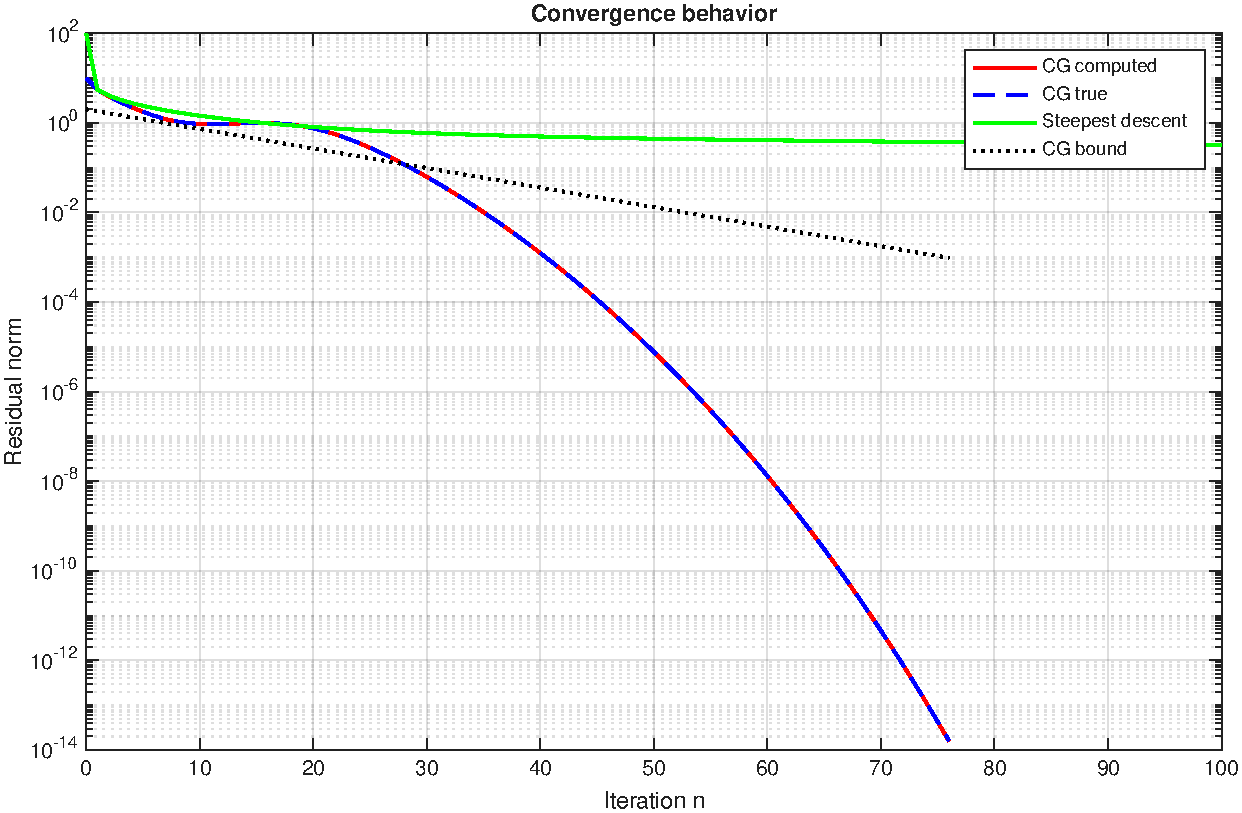
\includegraphics[width=0.7\textwidth]{convergence.pdf}
      \caption{Convergence behavior of the conjugate gradient method and the method of steepest descent for solving $Ax=b$. The figure shows the computed residual $\norm{r_n}_2$ and the true residual $\norm{b-Ax_n}_2$ for CG, the residual norm for steepest descent, and the theoretical convergence bound.}
      \label{fig:cg}
    \end{figure}
  \end{solution}

  \end{document}
